\subsection{Human Study on Quality-Diversity of Text Samples}\label{app:human_study_setup}
A study through human feedback lets us understand how well QD score performance through AI feedback translates to creating a high-quality, diverse set of creative texts from a subjective angle. We compare sets of human feedback evaluations for samples of diverse elites at the end of each run to measure translations from AI-assessed performance to human-assessed performance of methods in generating high-quality, diverse texts. In addition, the Human QD Score (sum of mean quality score for each category/label that is found in the set according to human feedback) gives us a rough understanding of how aligned quality-diversity improvement during the search is with the more subjective notion of quality-diversity; this score is low if the set deemed to cover a wide space of diverse texts from AI feedback fails to subjectively cover the space of desired diversity according to human evaluations. To distinguish between quality ratings from humans vs. AI feedback in this section, we refer to quality scores as those from human evaluators, and fitness scores as those from AI feedback.

To assess the robustness of quality and diversity measures in AI feedback, we carried out a study involving diverse elite samples selected from different bins of the QD archive from our tested runs. Over a total of 28 experiments (of which 4 are from embedding feedback experiment runs), five distinct stories per experiment are reviewed by six annotators. Each (generated) text was independently reviewed by two persons, resulting in a total of 280 annotations. 

During the annotation process, we collected a subjective assessment of the quality of the generation using a 5-point Likert scale based on the text quality in terms of flow, plot, presence of repetition, and correspondence to the study's topic. In addition, we assign each text to one of three categories. Two categories were specific to the study performed (such as positive/negative sentiment, romance/horror genre, or tragic/happy ending) and a third category was used when no element of the other two classes was identified.

We took action to prevent bias by presenting evaluators with texts to evaluate in a blind setting, with only the instructions for the study annotation task presented (to carefully read through the presented texts, then give a quality score and a label of the characteristic that best matches the texts). We provide the full set of results with caption descriptions from our human evaluation. In the \textbf{Opinions} domain, \crefrange{app:table_eval_opinions_b1}{app:table_eval_opinions_b4} contain the human evaluation results for sets from baseline methods, \crefrange{app:table_eval_opinions_aif_near_seeded}{app:table_eval_opinions_aif_replace_zero} contain the human evaluation results for sets from QDAIF methods, and \crefrange{app:table_eval_opinions_ef_near_seeded}{app:table_eval_opinions_ef_replace_zero} contain the human evaluation results for sets from embedding feedback QD methods. In the \textbf{Stories - Genre} domain, \crefrange{app:table_eval_stories_genre_b1}{app:table_eval_stories_genre_b4} contain the human evaluation results for sets from baseline methods, and \crefrange{app:table_eval_stories_genre_aif_near_seeded}{app:table_eval_stories_genre_aif_replace_zero} contain the human evaluation results for sets from QDAIF methods. For the \textbf{Stories - Ending} domain, \crefrange{app:table_eval_stories_ending_b1}{app:table_eval_stories_ending_b4} contain the human evaluation results for sets from baseline methods, and \crefrange{app:table_eval_stories_ending_aif_near_seeded}{app:table_eval_stories_ending_aif_replace_zero} contain the human evaluation results for sets from QDAIF methods.

We compiled the results of the full study in \cref{app:full_human_eval_tables}, and summarized the stats across the study in the paragraphs below.

\paragraph{Comparison of quality scores}
We observed that both annotators generally have a close agreement in their ratings with an average difference of 0.9 Likert points but there were occasional instances where they may differ by 2 or 3 units. These deviations occurred in 15\% and 5\% of the cases, respectively. This reflects that assessing the quality is somewhat subjective. To get a final estimation of the quality of the generated texts, the scores from both annotators were averaged.

\cref{fig:quality_vs_fitness} shows the average quality ratings from annotators for various ranges of fitness (here, the quality score obtained from AI feedback). The ranges were chosen in a way that ensured a similar amount of samples in each range. We observe clear evidence of a correlation between human and AI quality measures, indicating the usefulness of using AI feedback to assess quality. However, we also observed that fitness for the texts with the highest scores becomes uncorrelated to human-assessed quality. This implies that above a certain threshold, fitness is not a reliable measure of quality in some cases (and maybe slightly lower fitness solutions were preferred by humans). Therefore, we suggest that in future work, more research is done in studying the relationship between (high-confidence) evaluations from AI feedback, and reward hacking of solutions \citep{nguyen2015deep,skalse2022defining,lehman2019surprising} under certain conditions and controls during the search (e.g. through the use of seed texts for human-preferred outputs, as shown in \cref{table:mean_human_eval_baselines_vs_aif}, or additional constraints on the generated solutions during search \citep{lehman2010revising,brant2017minimal}).

\begin{figure}[t]
    \centering    
    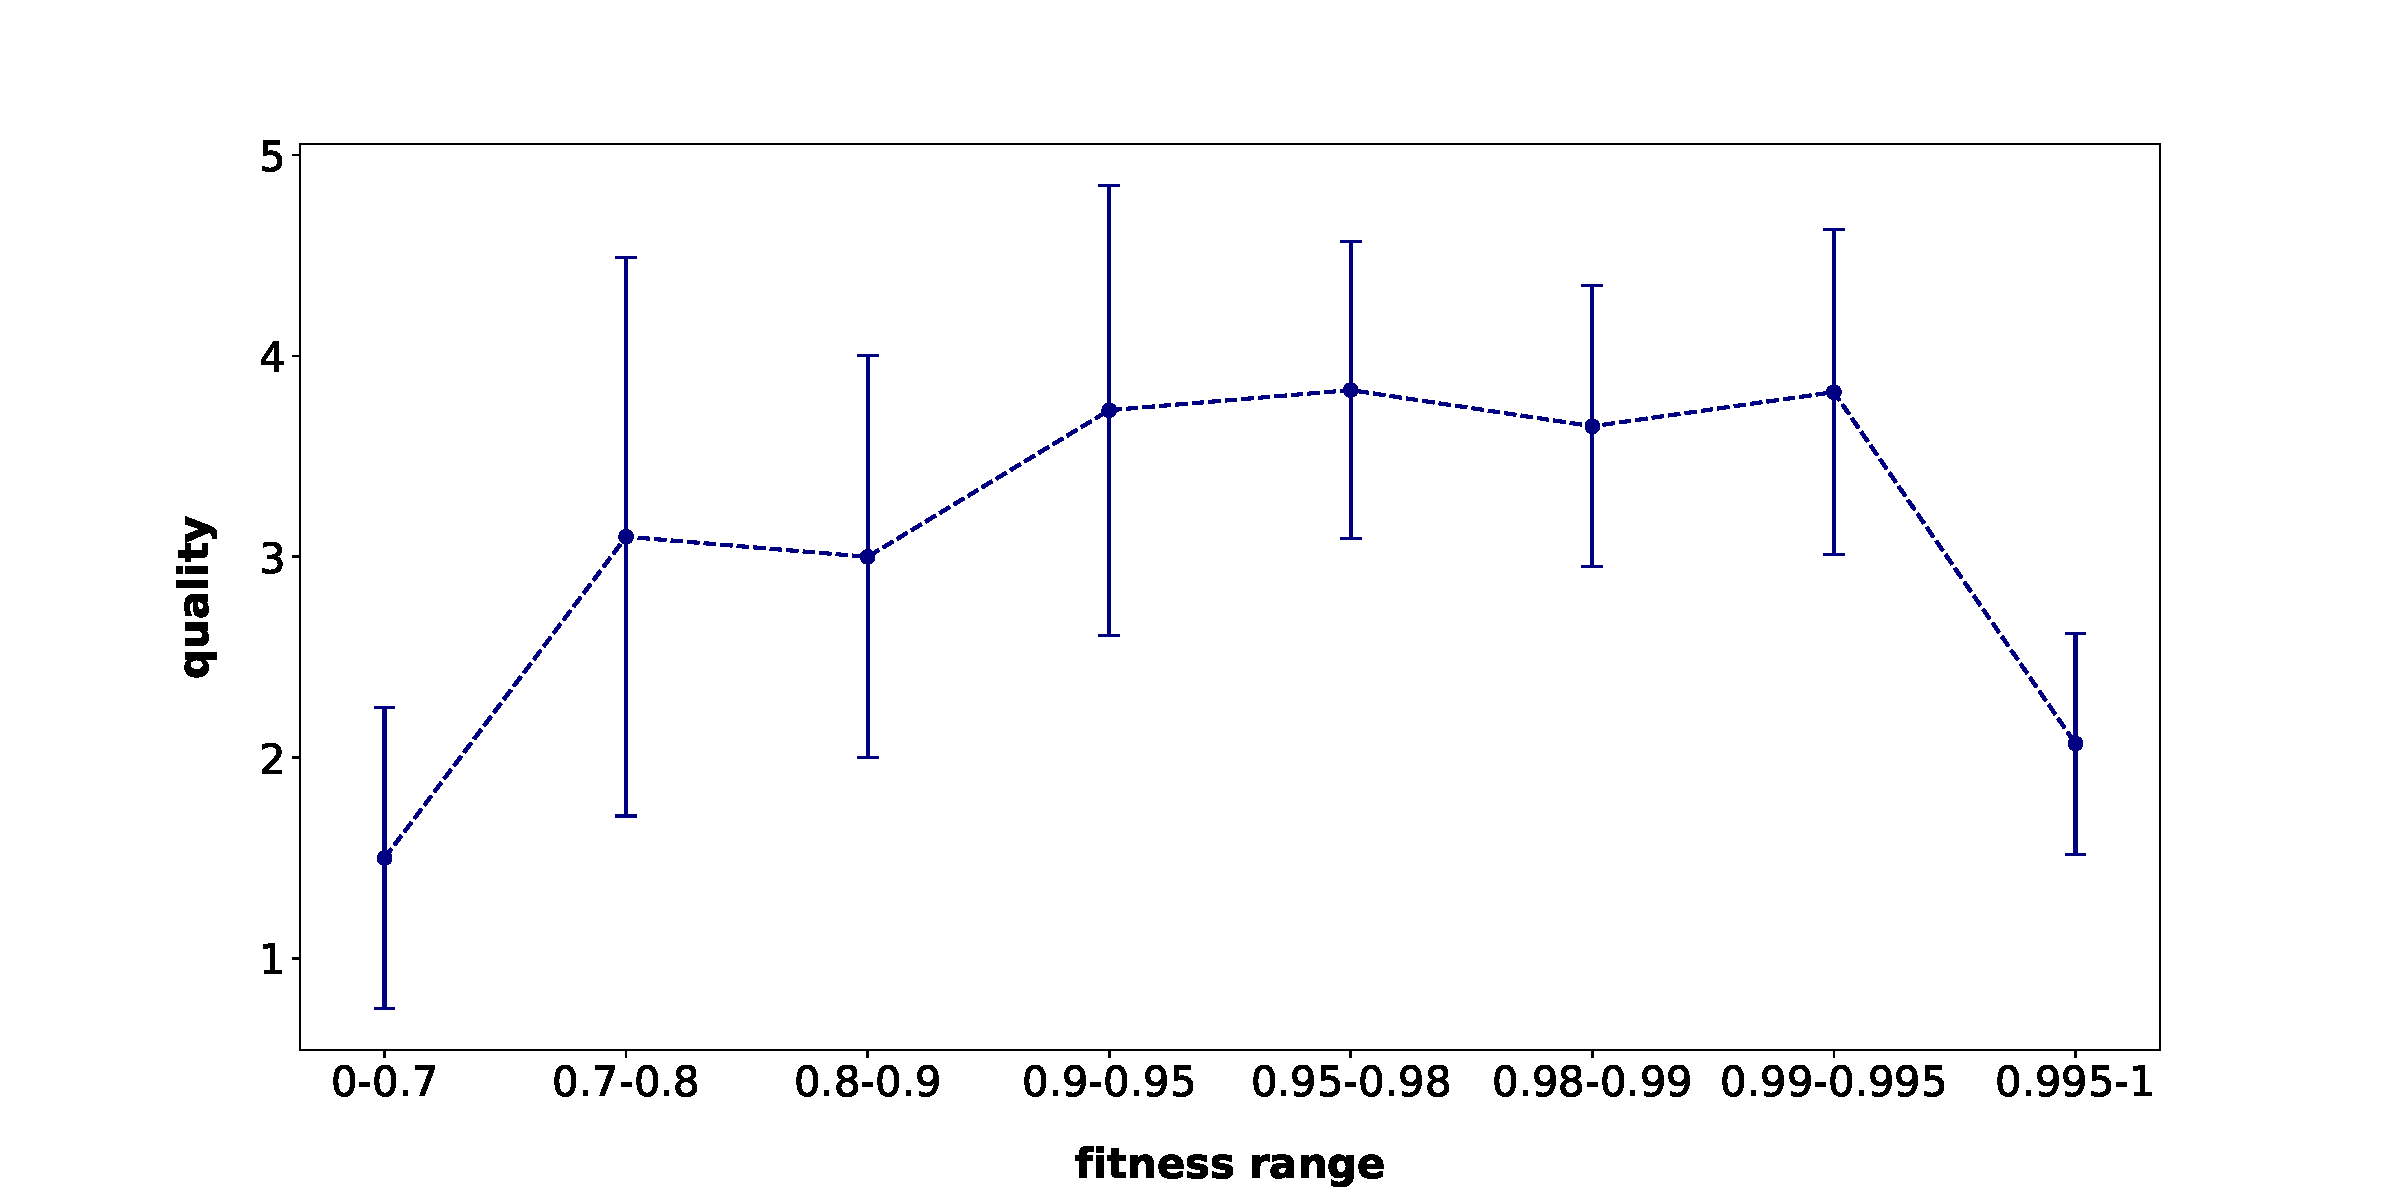
\includegraphics[width=\textwidth]{main_figures/quality_vs_fitness.pdf}
    \caption{\textbf{Correlation plot between quality rating from human annotators, and fitness range (quality computed from AI feedback).} Mean human-annotated quality and statistical error for different ranges of AI feedback fitness scores indicate more frequent instances of reward hacking \citep{skalse2022defining,lehman2019surprising} from the outputs of some search methods evaluated in this study.} 
    \label{fig:quality_vs_fitness}
\end{figure}


\paragraph{Comparison of diversity measurements}
For diversity, we observed that the two annotators agreed on the classification of a generated text in the same category 73 percent of the time. On the AI feedback side, diversity is collected on a 20-bin axis, measuring different degrees of correspondence to two experiment-specific categories mentioned earlier. For the purpose of comparison with human feedback, these bins are clustered into a first category (bins 0 to 8), a second category (bins 11 to 19) and a neutral category (bins 9 and 10). Additionally, the 5 samples for each set were collected from a relatively uniform spread of bins from one end of the diversity axis to another (specifically, bins in set [0, 6, 9, 13, 19], except for when the method fails to find a solution for the bin, then the next closest solution near the bin is chosen). This arbitrary arrangement allows for a relatively uniform distribution among the three categories.

On average, AI feedback agrees with a human annotator on the text category label 73\% of the time. On samples where both annotators agree on the label of the text, this agreement rate increases to 82\%. Within this set, the agreement increases to 95\% on samples when we look at samples where both annotators give a label that is not the neutral category. For some samples from bins 6 and 13, one human annotator gave a neutral label and the other annotator one of the other two labels (closer to the AI feedback diversity measure for these bins), indicating that some samples lie between neutral and extreme in the given measure. These findings suggest that diversity classification from AI feedback is relatively reliable, especially in texts where humans agree on the label.

\paragraph{Baseline quality rating.}
The average quality score given by annotators for a given sample was 3.18, close to the middle rating of 3. This gives us an indication of what could be considered the threshold for subjectively good or bad outputs.

The average human (subjective) QD score of all sets in the study is 0.606. This is another indication for the threshold for determining which set from a given run/method had high-quality, diverse texts.

